
\subsection{Análises}

Nesta secção efetuaremos scans ao servidor apache na máquina virtual metasploitable que corre o mutillidae.\newline

\par Os exemplos de testes que figuram neste relatório, estao divididos em duas categorias, exemplos básicos e exemplos avançados e são:
\begin{itemize}
  \item Exemplos Básicos:
  \begin{itemize}
    \item Spider a website
    \item Fuzz a website
    \item Scan Ativo
    \item Mapear websites autenticados com Ajax
  \end{itemize}

  \item Exemplos Avançados:
  \begin{itemize}
    \item SQL Injections
    \item Brute Force
    \item Cross Site Scripting
    \item Obter ficheiros escondidos no Servidor
  \end{itemize}
\end{itemize}



%################################################################################################


%##################################### BASIC EXEAMPLES ##########################################


%################################################################################################




%######################################### SPIDER ###############################################


\subsubsection{Spider a website}

Spider é um scan passivo e inofencivo destinado a procurar em pedidos e respostas falhas como security headers ou anti CSRF tokens em falta. 
Vamos então realizar esta procura passiva fazendo uso do ZAP.
\begin{figure}[H]

  \centering

  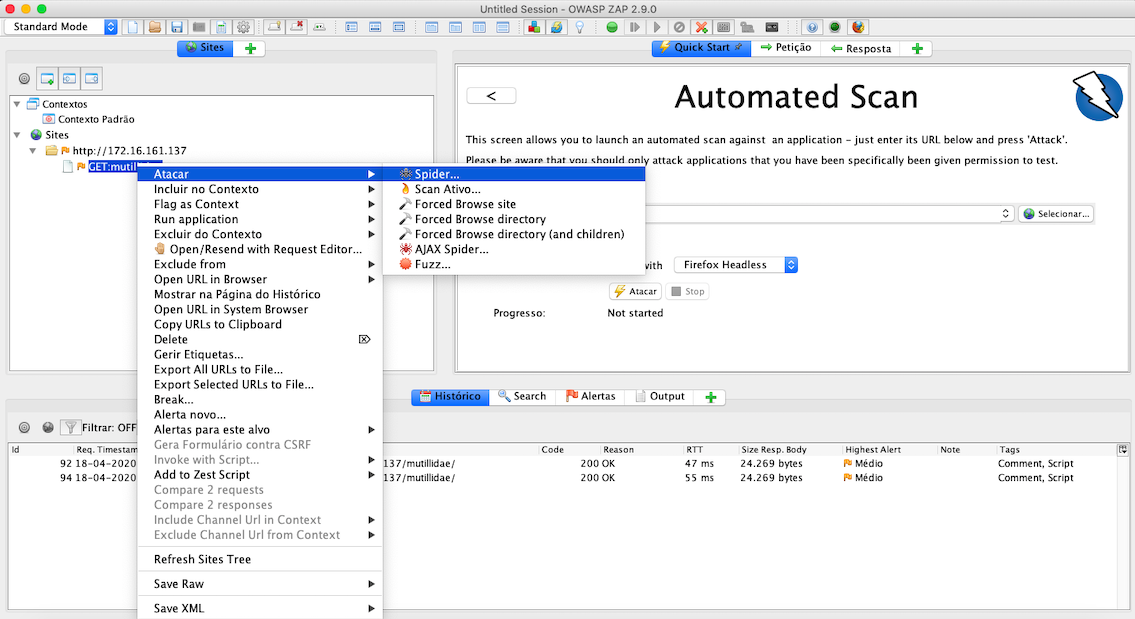
\includegraphics[scale = 0.31]{fig11.png}

  \caption{Procedimento para realizar um Spider Scan}

\end{figure}

Após termos realizado este procedimento podemos ver uma alteração na janela que mostrava os sites vistos.
\begin{figure}[H]

  \centering

  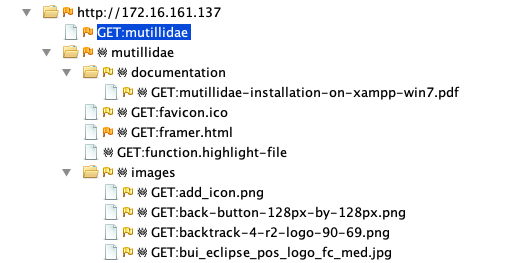
\includegraphics[scale = 0.31]{fig12_1.png}
  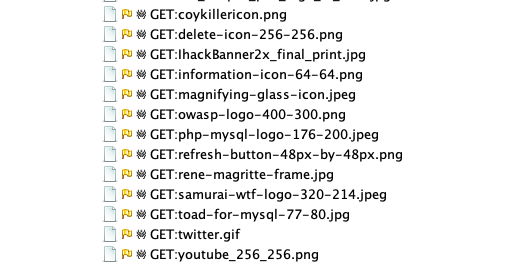
\includegraphics[scale = 0.31]{fig12_2.png}
  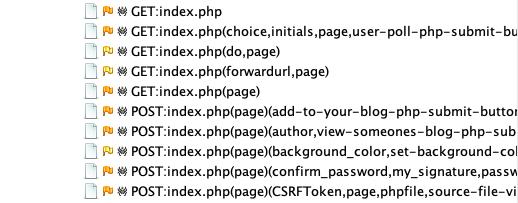
\includegraphics[scale = 0.31]{fig12_3.png}

  \caption{Resultado do Spider Scan}

\end{figure}


A cor da bandeira ao lado dos pedidos indica falhas na resposta recebida, quanto mais escura a cor mas grave é a falha.
Também há uma janela onde são reportados os alertas para melhor visualização dos problemas. Em baixo podemos ver o conteúdo dessa janela.
\begin{figure}[H]

  \centering

  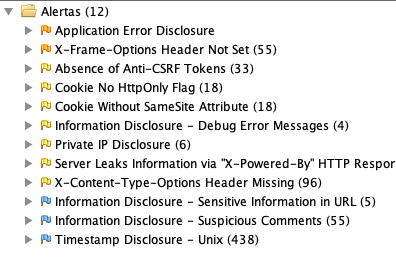
\includegraphics[scale = 0.31]{fig12_4.png}

  \caption{Alertas resultantes do Scan}

\end{figure}

%######################################### Fuzzering ##############################################


\subsubsection{Fuzz a website}


Para fins demonstrativos vamos usar a página de login para realizar o ataque fuzz. Nas figuras segunites vemos o resultado de tentar fazer login no servidor mutillidae com o username \textit{admin} e a password \textit{wrongPassword} bem como o respetivo pedido apanhado pelo ZAP.
\begin{figure}[H]

  \centering

  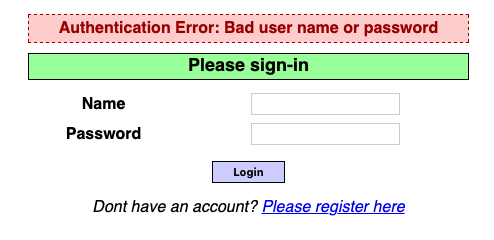
\includegraphics[scale = 0.31]{fig22.png}

  \caption{Formulario de autenticação}

\end{figure}
\begin{figure}[H]

  \centering

  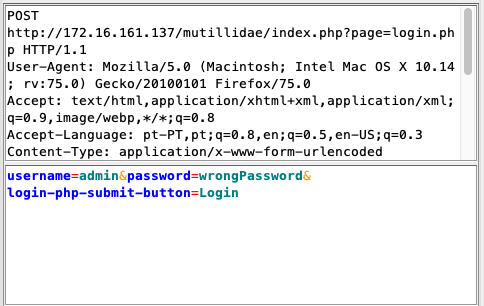
\includegraphics[scale = 0.31]{fig23.png}

  \caption{Pedido de autenticação submetido}

\end{figure}

Agora para realizarmos o fuzz temos de selecionar o pedido apanhado pelo ZAP com o username e a password errados e fazendo uso das opções disponibilizadas pelo botão direito do rato escolher Fuzz.

\begin{figure}[H]

  \centering

  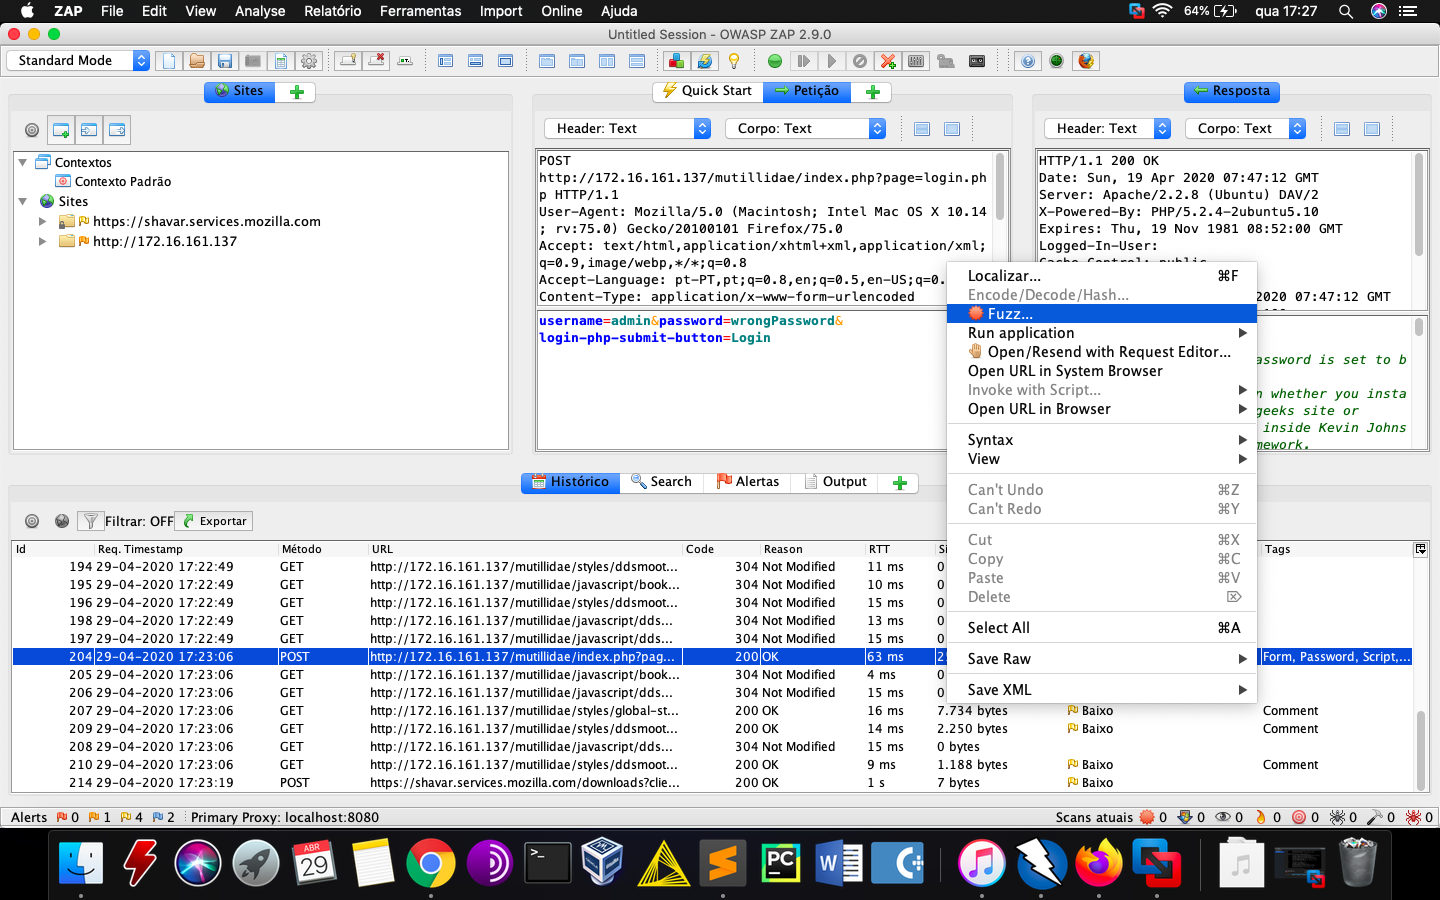
\includegraphics[scale = 0.31]{fig24.png}

  \caption{Abertura da janela de configuração do Fuzzer}

\end{figure}

Agora com a janela do fuzz aberta basta-nos selecionar o campo sobre o qual queremos executar o fuzz na mensage interceptada e carregar um payload para substituição. Neste caso como estamos a falar de um autenticaçao vamos escolher a opção \textit{File Fuzzers} e dentro desta escolher \textit{injeção SQL} e dentro de todas as opções vamos escolher apenas duas para manter o teste simples. Note-se que na segunda figura podemos ver no campo \textit{Payloads Preview} onde é mostrado o que será registado no campo.

\begin{figure}[H]

  \centering

  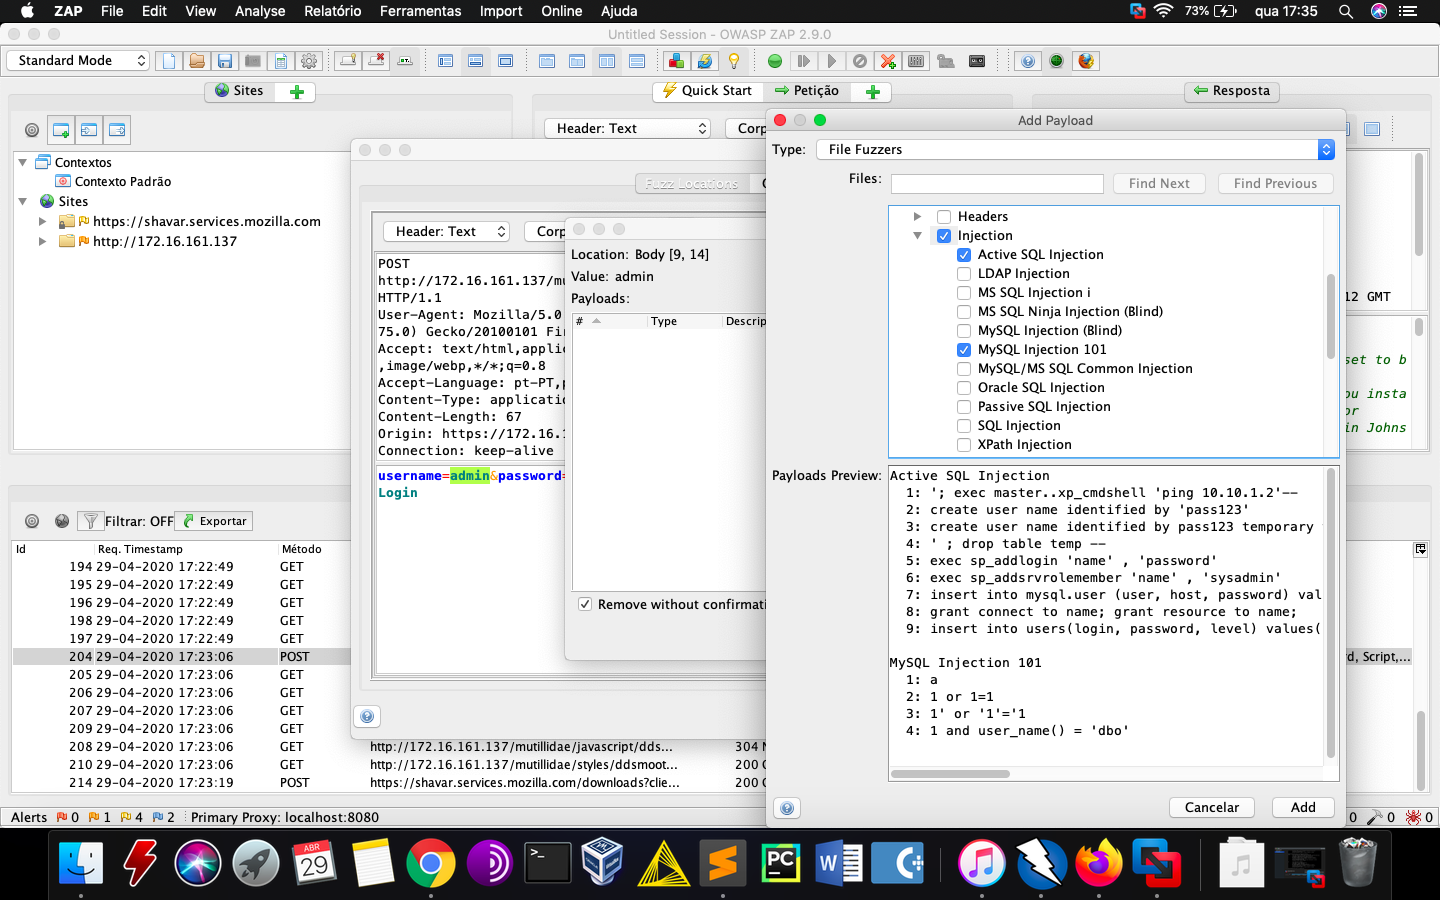
\includegraphics[scale = 0.31]{fig26.png}

  \caption{Configuração escolhida para o Fuzzer}

\end{figure}

Após escolhermos as opções basta carregar no botão \textit{Start Fuzzer} e esperar. Como o fuzzer executa rápido obtemos respostas que podem ser ordenadas pelo tamanho de corpo de resposta e nas quais podemos ver o payload. Para uma busca mais eficaz podemos usar a barra search sobre o tipo \textit{HTTP Fuzzer Results} para procurar palavras especificas como \textit{error} ou \textit{syntax}. Neste caso usamos a palavra syntax e se repararmos temos o campo username substituido por uma pelica, o que causa um erro no servidor. Se fizermos a substituição e submetermos o formulário de login na página acabamos por confirmar a existencia de um erro como se vê nas figuras abaixo.

\begin{figure}[H]

  \centering

  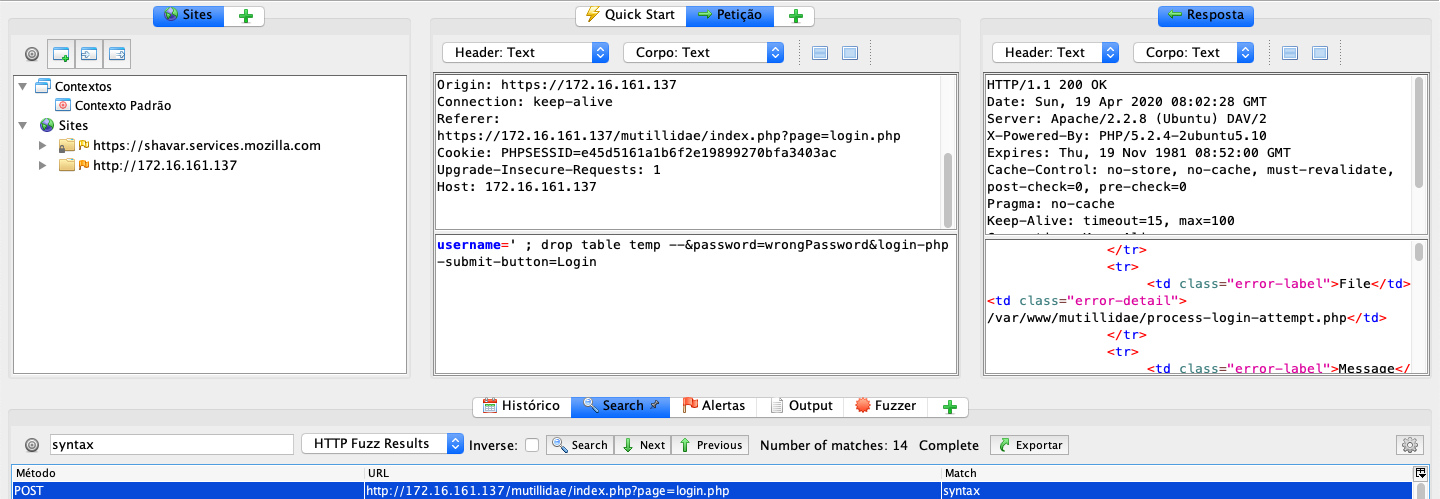
\includegraphics[scale = 0.31]{fig28.png}

  \caption{Exemplo de substituição do username}

\end{figure}
\begin{figure}[H]

  \centering

  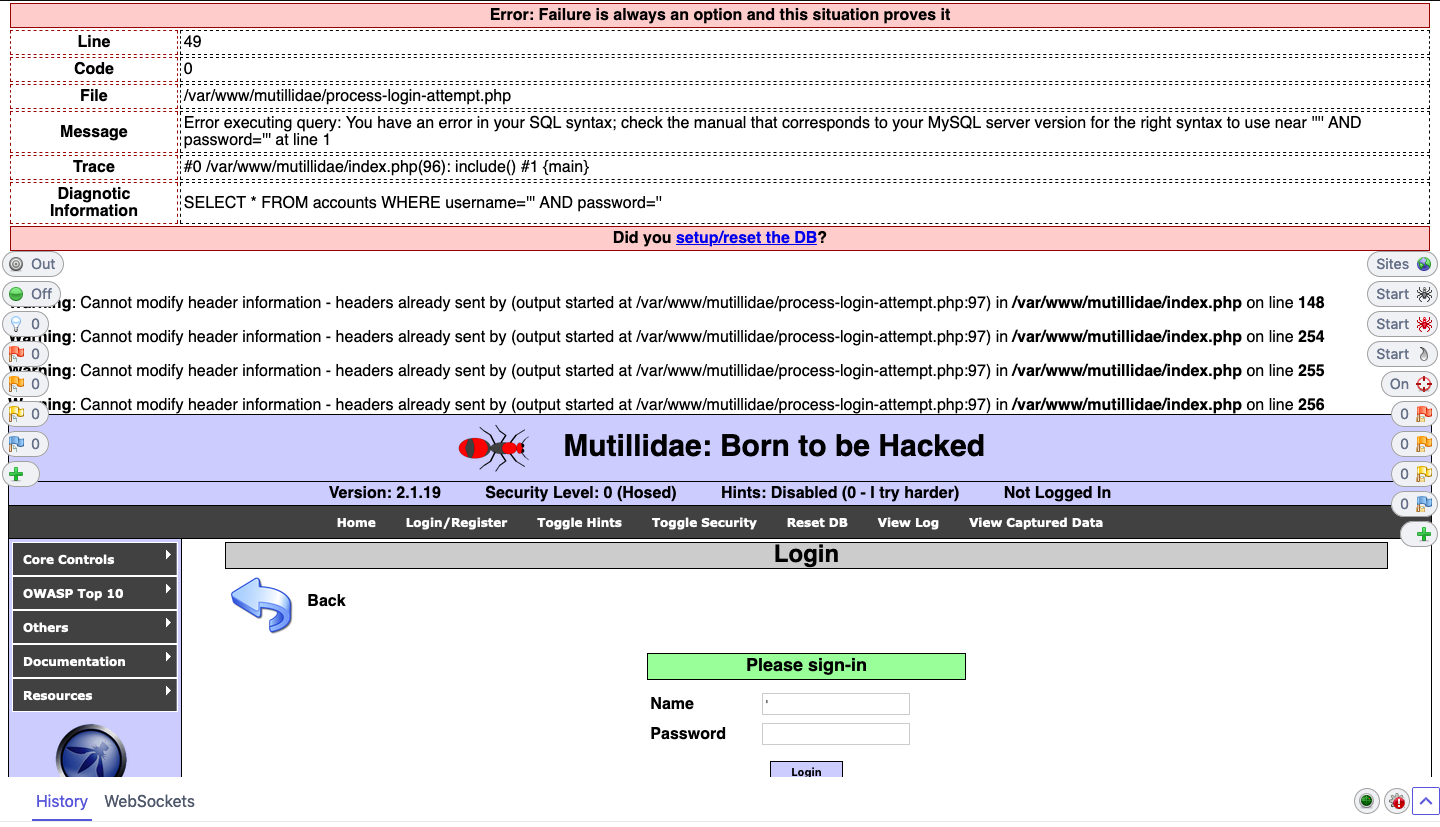
\includegraphics[scale = 0.31]{fig29.png}

  \caption{Resultado da substituição do username}

\end{figure}

Para além disso note-se também que obtivemos informação útil sobre a base de dados. Agora sabemos que existe uma tabela SQL chamada accounts com os campos username e password.



\subsubsection{Scan ativo}

Para fazer o scan ativo basta-nos simplesmente escolher um site e selecionar a opção scan ativo, este correrá um scan padrão pré-definido no ZAP.

\begin{figure}[H]

  \centering

  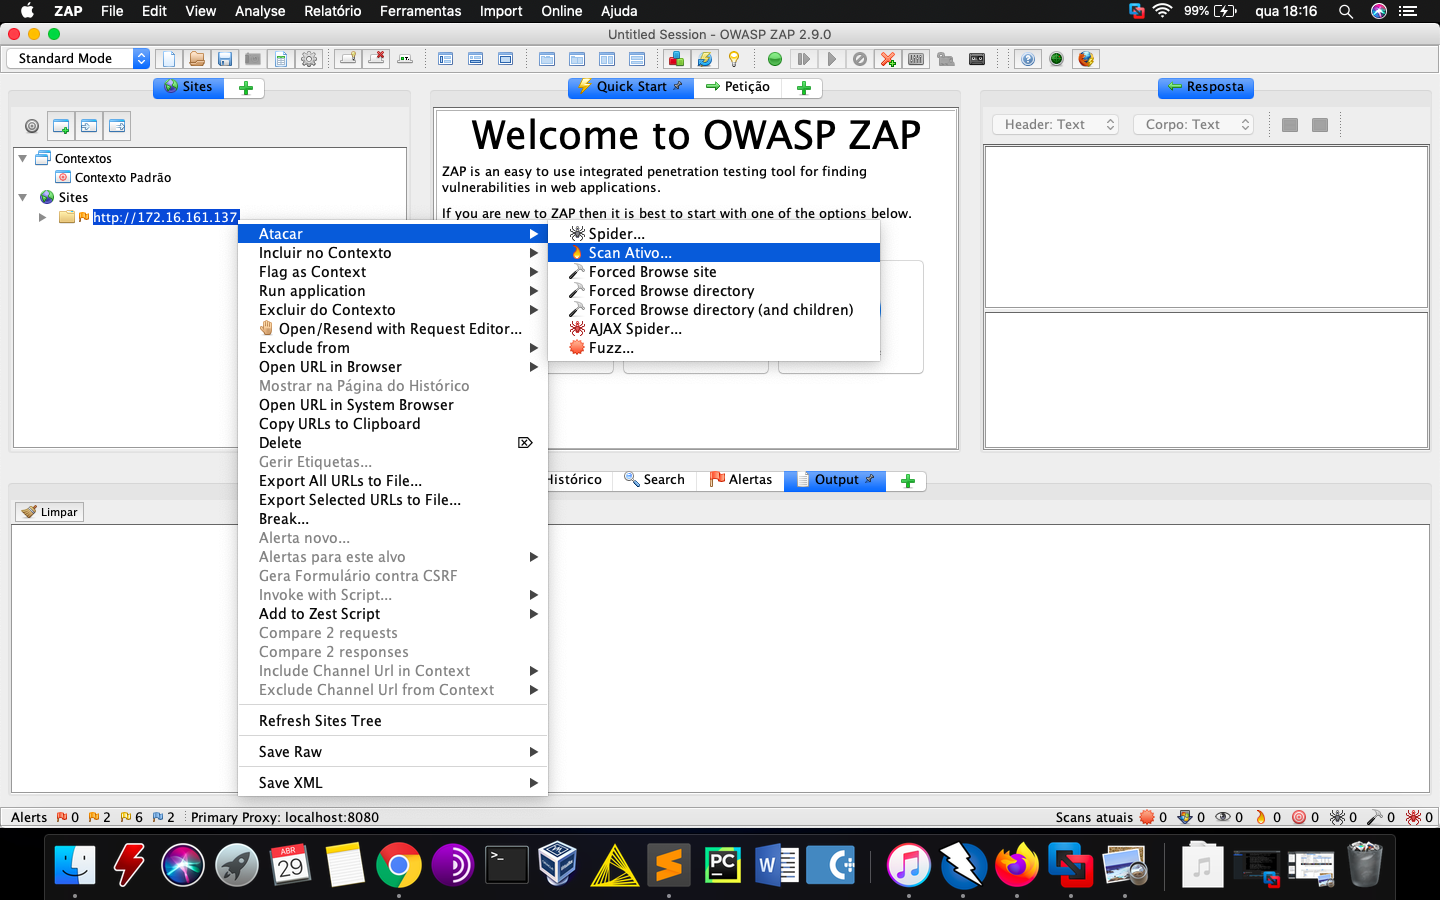
\includegraphics[scale = 0.31]{fig34.png}

  \caption{Procedimento para realizar um Scan Ativo}

\end{figure}


 Podemos ver o resultado do mesmo na figura abaixo, onde na tab Alertas obtemos todos os alertas que o scan padrão detetou etiquetadas pela gravidade da falha identificada pela cor da bandeira.

\begin{figure}[H]

  \centering

  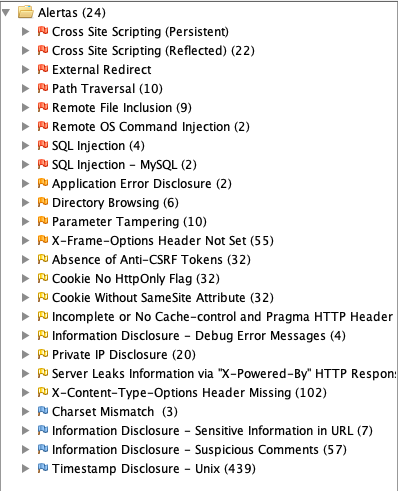
\includegraphics[scale = 0.31]{fig17.png}

  \caption{Alertas resultantes de realizar um Scan ativo}

\end{figure}


%###################################### AJAX ############################################


\subsubsection{Mapeamento de websites com autenticação de utilizador usando Ajax}

A vantegem desta técnica de Spider é podermos aceder a URLs aos quais apenas utilizadores autenticados podem aceder, originando assim um mapeamento mais detalhado da organização do site.\newline
O primeiro passo para realizar este teste é ter descoberto uma combinação username-password válida e realizar a autenticação. Caso ainda não tenha realizado este passo por favor veja a subsecção de Brute Force.\newline
Para garantir que se está auntenticado caso observemos a tab HTTP session devemos ver uma imagem parecida com a seguinte.\newline

\begin{figure}[H]

  \centering

  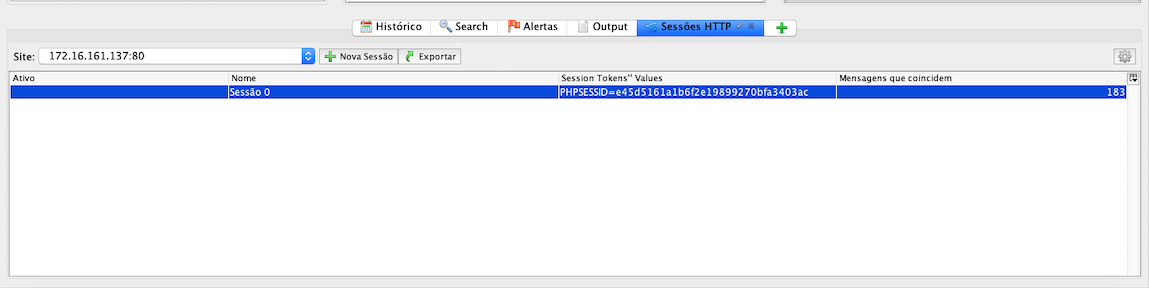
\includegraphics[scale = 0.31]{fig35.png}

  \caption{Sessão HTTP por ativar}

\end{figure}

Devemos então clicar na barra correspondente á seção atual na janela e definir a mesma como ativa. Posteriormente na janela onde visualizamos os sites visitados devemos selecionar aquele com a sessão ativa e escolher a opção \textit{Ajax Spider}. Desta forma o Ajax usará a nossa conta para realizar o Spider do website. Para além disso o Ajax Spider reautentica-se para garantir que caso exista a opção de \textit{log off} o utilizador não seja desconectado.

\begin{figure}[H]

  \centering

  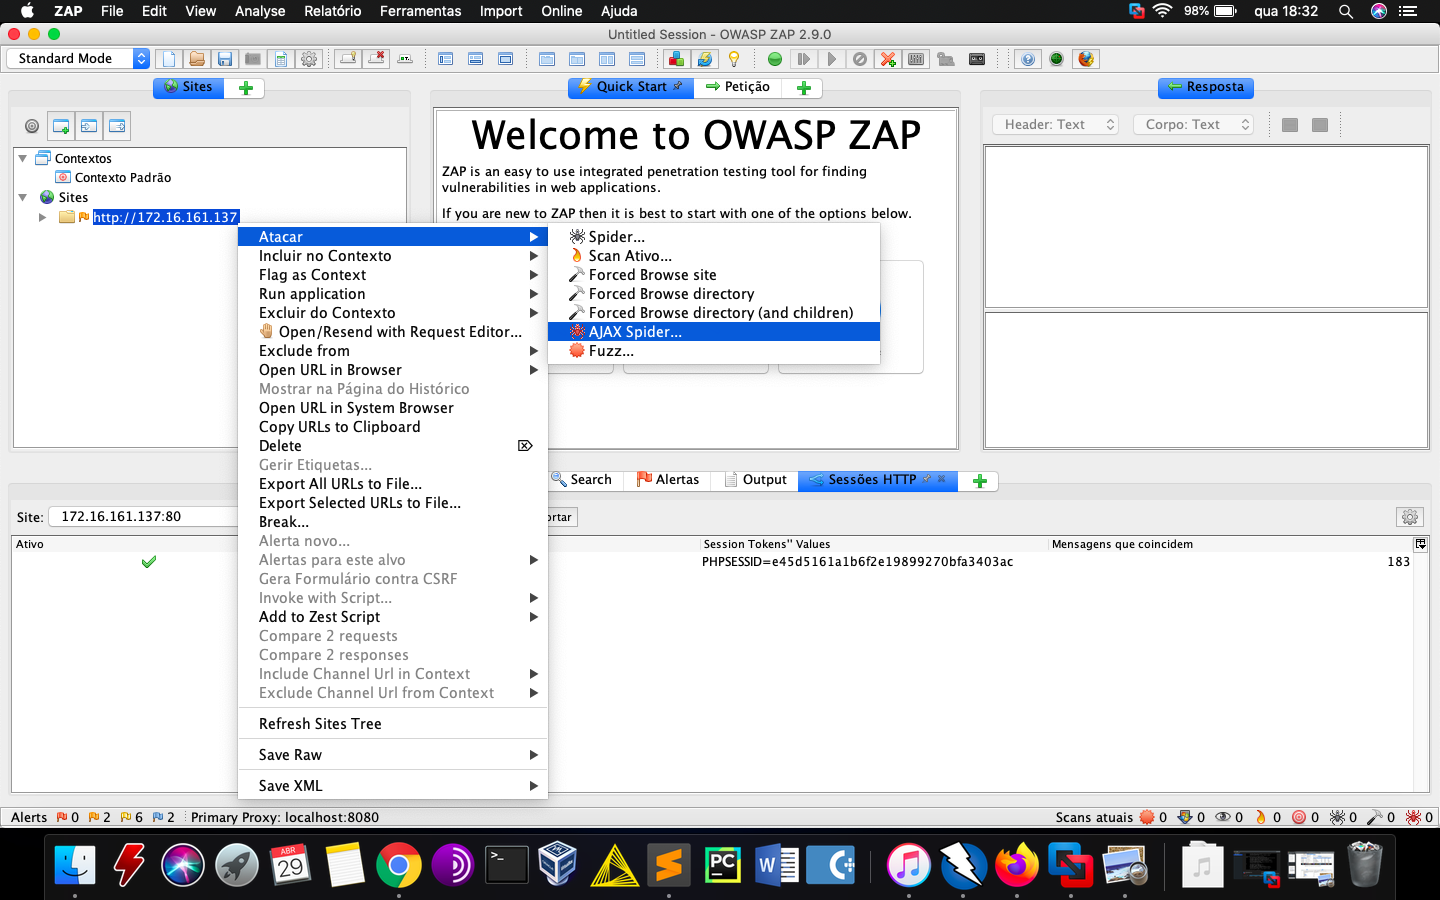
\includegraphics[scale = 0.31]{fig36.png}

  \caption{Procedimento para realizar um mapeamento com Ajax após ativação da sessão}

\end{figure}

Por fim podemos ver os pedidos realizados pelo \textit{Ajax} na janela inferior do ZAP bem como aceder á configuração do site alvo na tab correspondente aos sites.  

\begin{figure}[H]

  \centering

  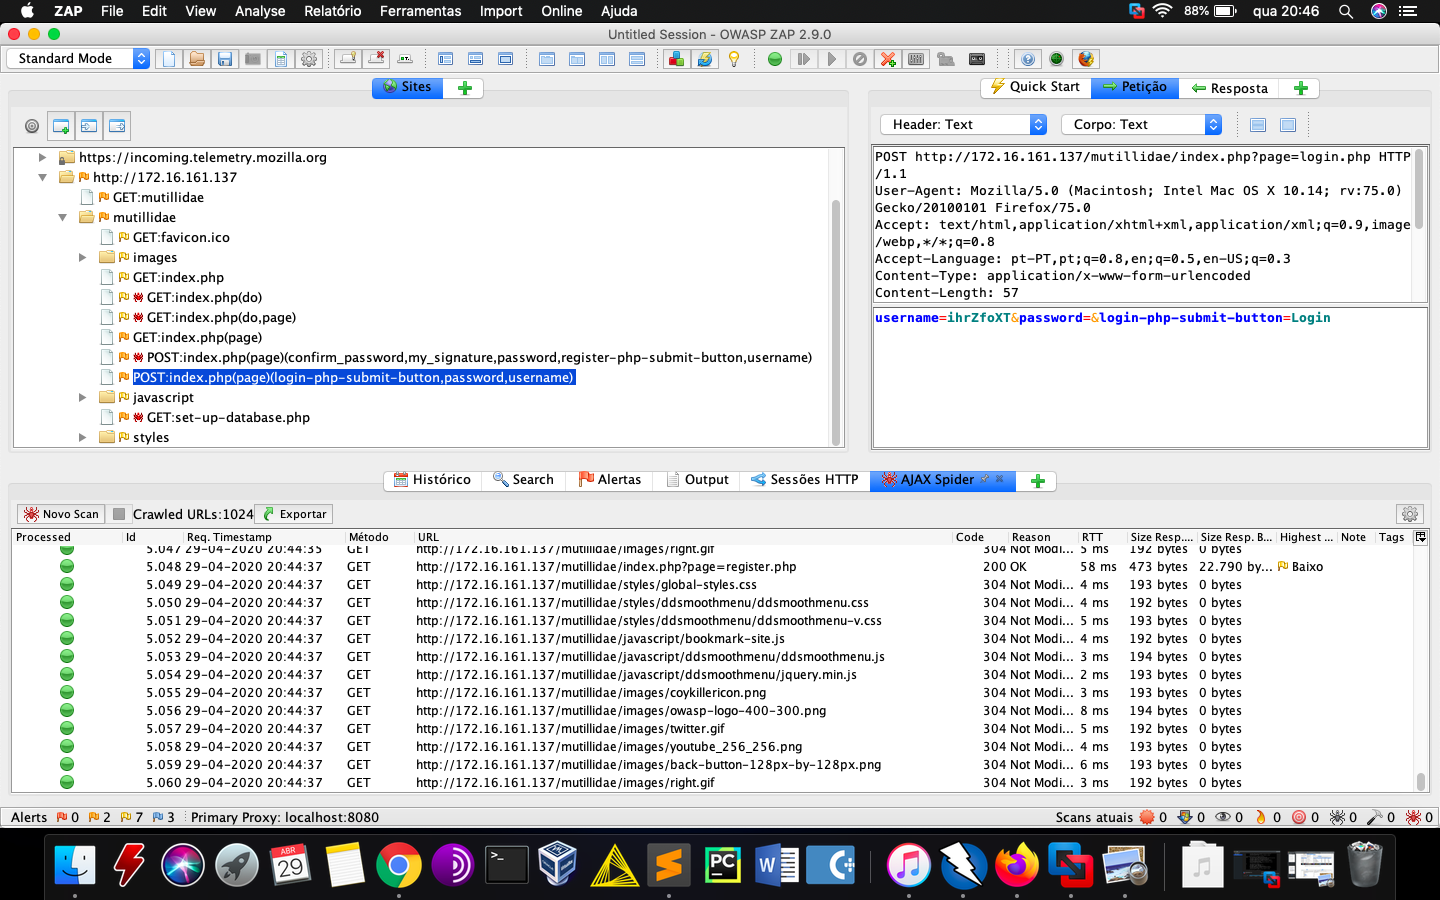
\includegraphics[scale = 0.31]{fig37.png}

  \caption{Site mapeado e pedidos feitos pelo Ajax}

\end{figure}




%################################################################################################


%################################### ADVANCED EXEAMPLES #########################################


%################################################################################################


\subsubsection{SQL Injections}

O propósito deste exemplo e demonstrar como injeções de código SQL podem comprometer a segurança. Primeiro vamos autenticar-nos no site e executar um scan ativo para testar o mesmo, como o ZAP esteve a guardar tudo em background ao executar o scan pode revelar mensagens interessantes. Como se pode ver na imagem temos 2 alertas de possiveis injeções de código SQL.




\begin{figure}[H]

  \centering

  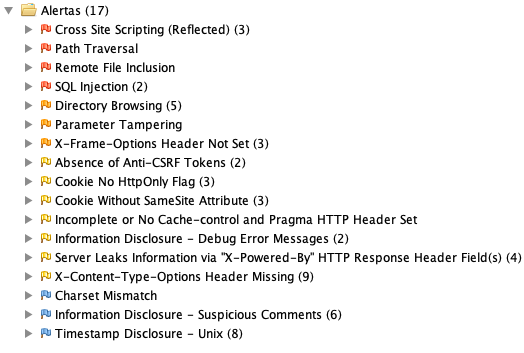
\includegraphics[scale = 0.31]{fig39.png}

  \caption{Alertas resultantes do Scan Ativo}

\end{figure}

Se nos aprofundarmos nos alertas podemos inspecionar o alerta e obter mais informação sobre a falha.


\begin{figure}[H]

  \centering

  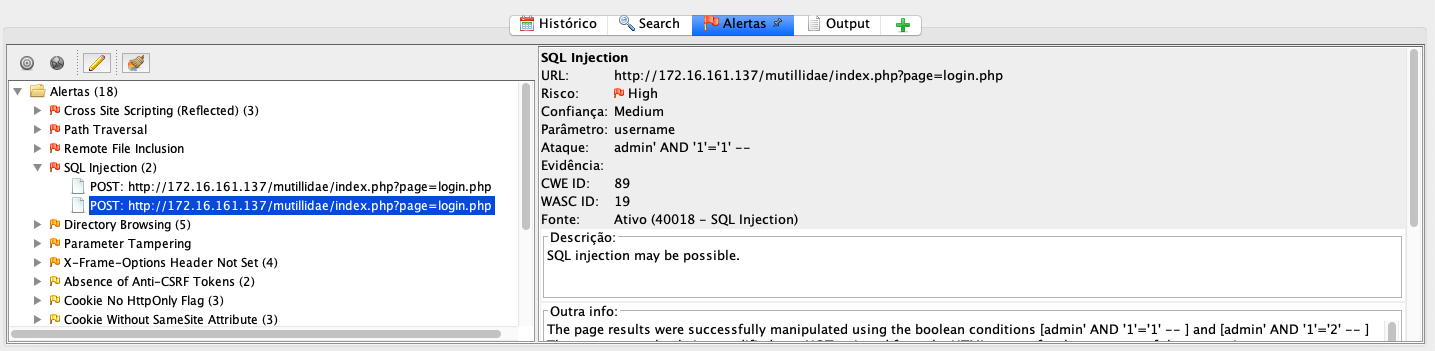
\includegraphics[scale = 0.31]{fig40.png}

  \caption{Alertas de SQL injection}

\end{figure}


Agora, basta-nos selecionar o campo do username e selecionar Fuzzer. No Fuzzer basta-nos adicionar uma nova \textit{Fuzzer Location} carregando no botão add na janela do \textit{Fuzzer}. Em seguida escolhemos todos os tipos de injeções MySQL, começando em seguida o scan. 


\begin{figure}[H]

  \centering

  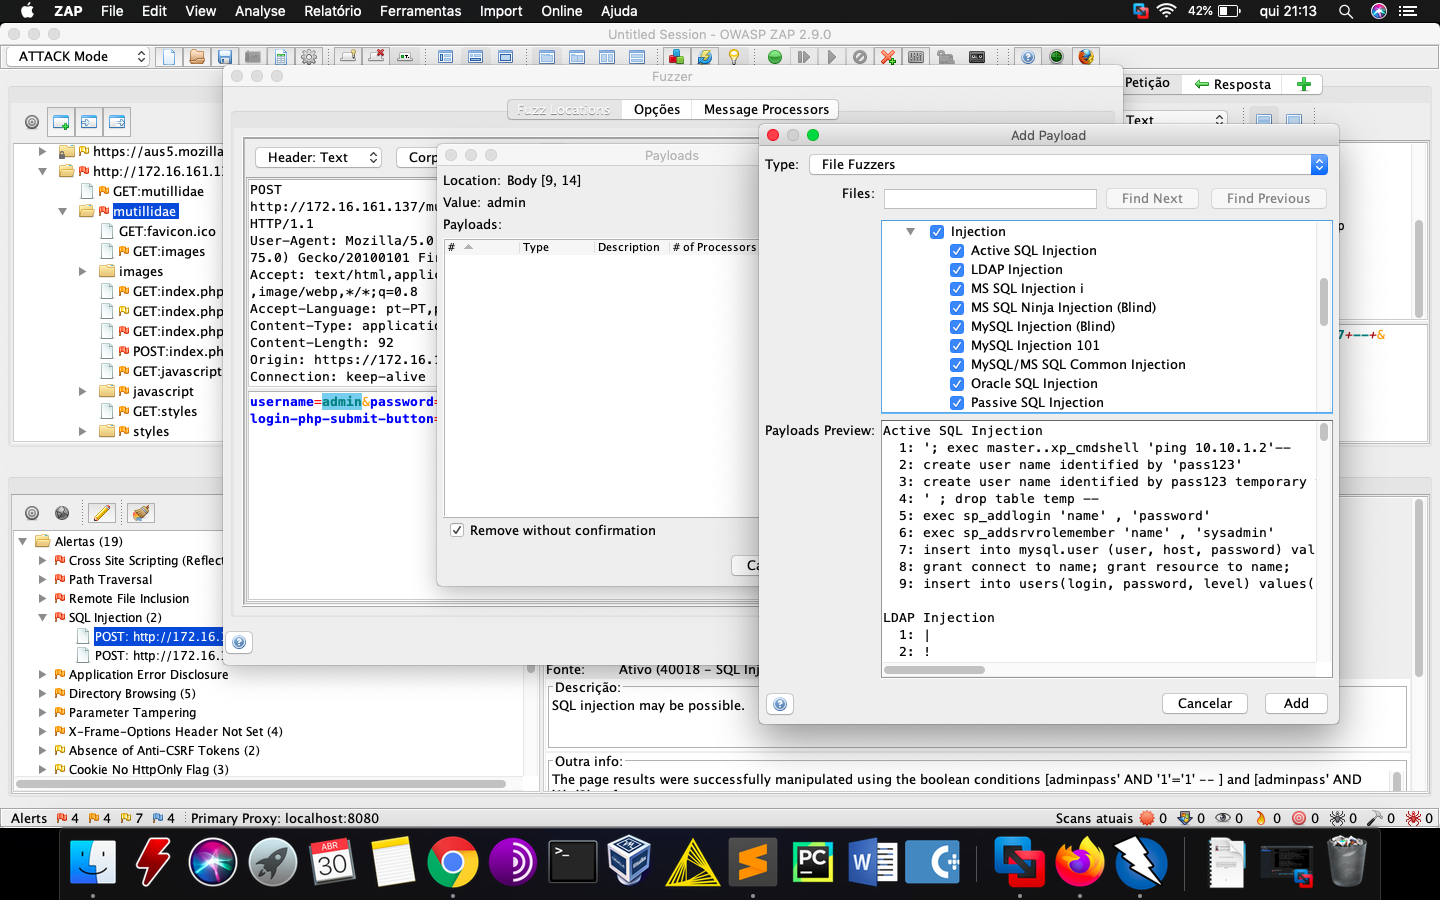
\includegraphics[scale = 0.31]{fig41.png}

  \caption{Configuração do Fuzzer para Injeção de código SQL}

\end{figure}



Se olharmos para uma das mensagens etiquetada com a tag \textit{"Found"}, podemos ver o que o ZAP enviou no formulário. No caso da mensagem que podemos visualizar em baixo foi inserido no campo admin o código: \textit{' or '1'='1}.

\begin{figure}[H]

  \centering

  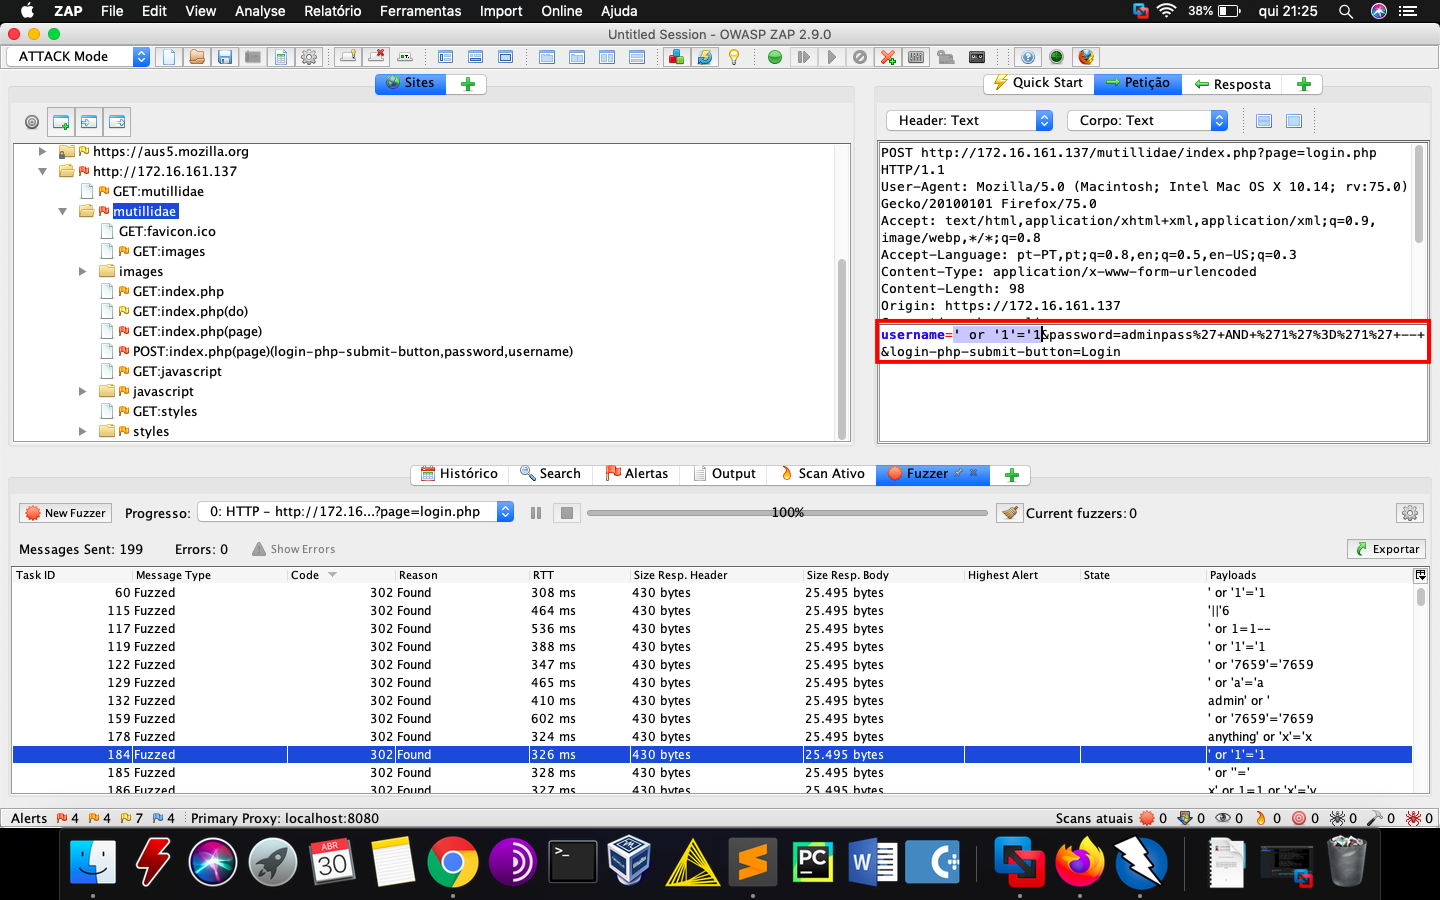
\includegraphics[scale = 0.31]{fig42.png}

  \caption{Exemplo de injeção SQL bem sucedida}

\end{figure}

Se testarmos este código no campo do admin conseguimos acesso ao site.

\begin{figure}[H]

  \centering

  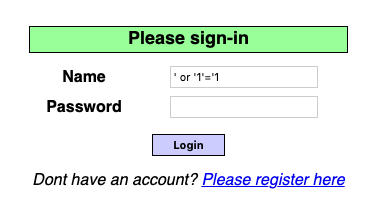
\includegraphics[scale = 0.31]{fig43.png}

  \caption{Injeção de código SQL manual}

\end{figure}
\begin{figure}[H]

  \centering

  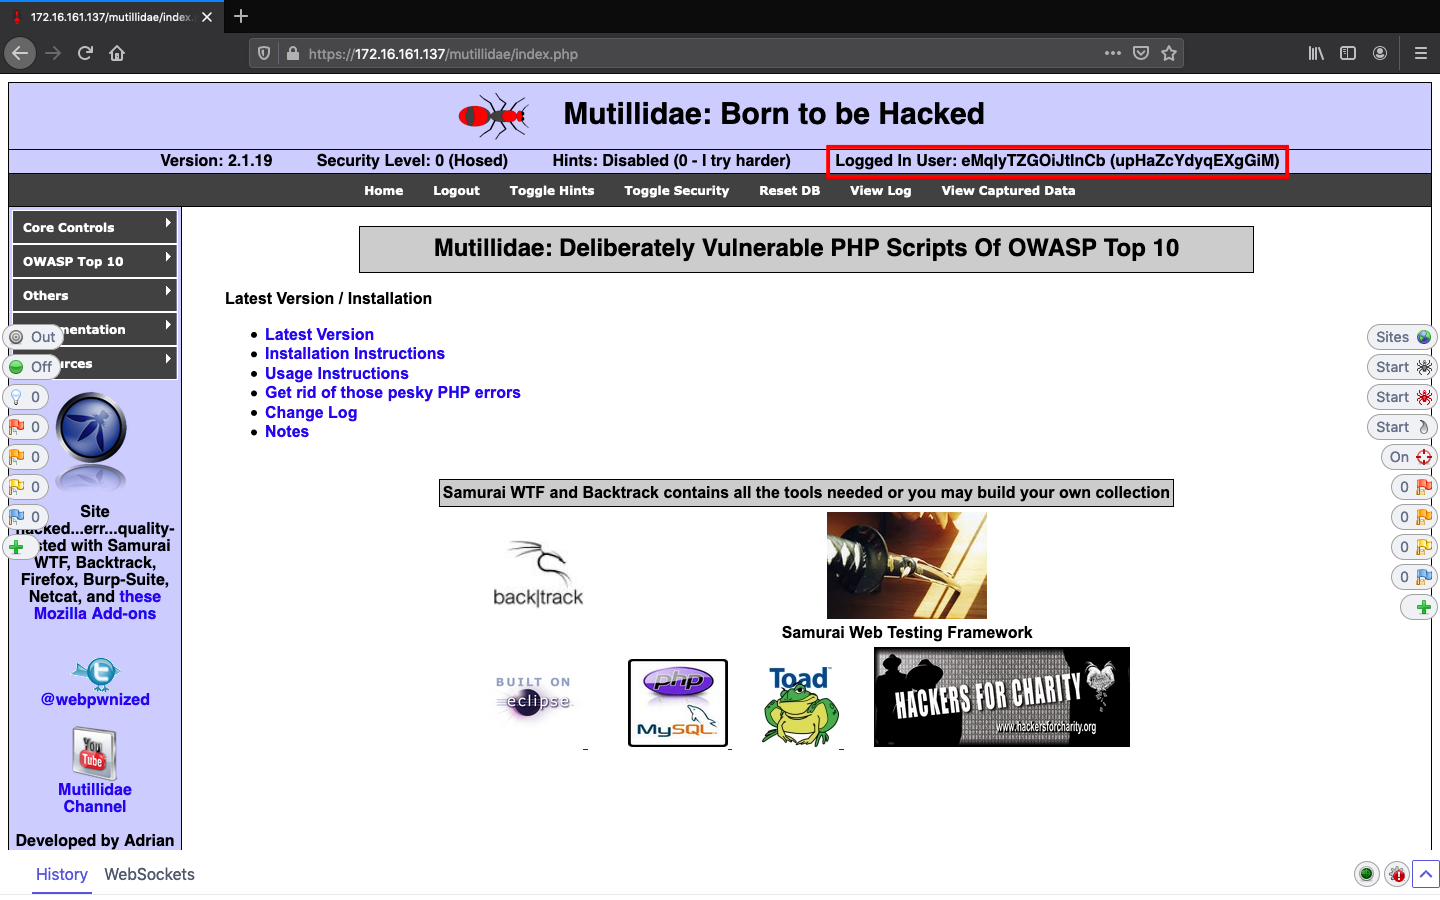
\includegraphics[scale = 0.31]{fig44.png}

  \caption{Login bem sucedido com injeção SQL}

\end{figure}

A lição a tirar neste teste é que não é feita nenhuma verificação do que foi inserido pelo utilizador, ou seja quem desenvolveu o acesso á base de dados confia cegamente no input fornecido pelo utilizador o que permite ataques deste tipo.





\subsection{Ataque Brute Force}

Antes de executarmos este ataque é importante lembrar que este é um teste que demora bastante tempo a executar, por isso convem estar atento a mensagens que aguns sites dão como este \textit{utilizador não existe} ou \textit{password inválida}, que nos dão pistas sobre se devemos respetivamente mudar o username ou tentar passwords diferentes visto que o username existe na base de dados. Por isso devemos começar por tentar obter um username. Digamos que o username que identificamos é : \textit{admin}.
Para executar este ataque á semelhança do exemplo usado com o Fuzzer devemos colocar  no campo de username o username válido e submeter o formulário. Para melhor compreenção o campo password será preenchido com a palavra \textit{"Altera-me"}.
Neste caso tal como no fuzz selecionamos o pedido interceptado e usamos a opção Fuzzer. Na mensagme selecionamos a palavra \textit{Altera-me} e adicionamos um ficheiro pré-gerado com palavras que podem ser uma password correta: \textit{passwords.txt}.


\begin{figure}[H]

  \centering

  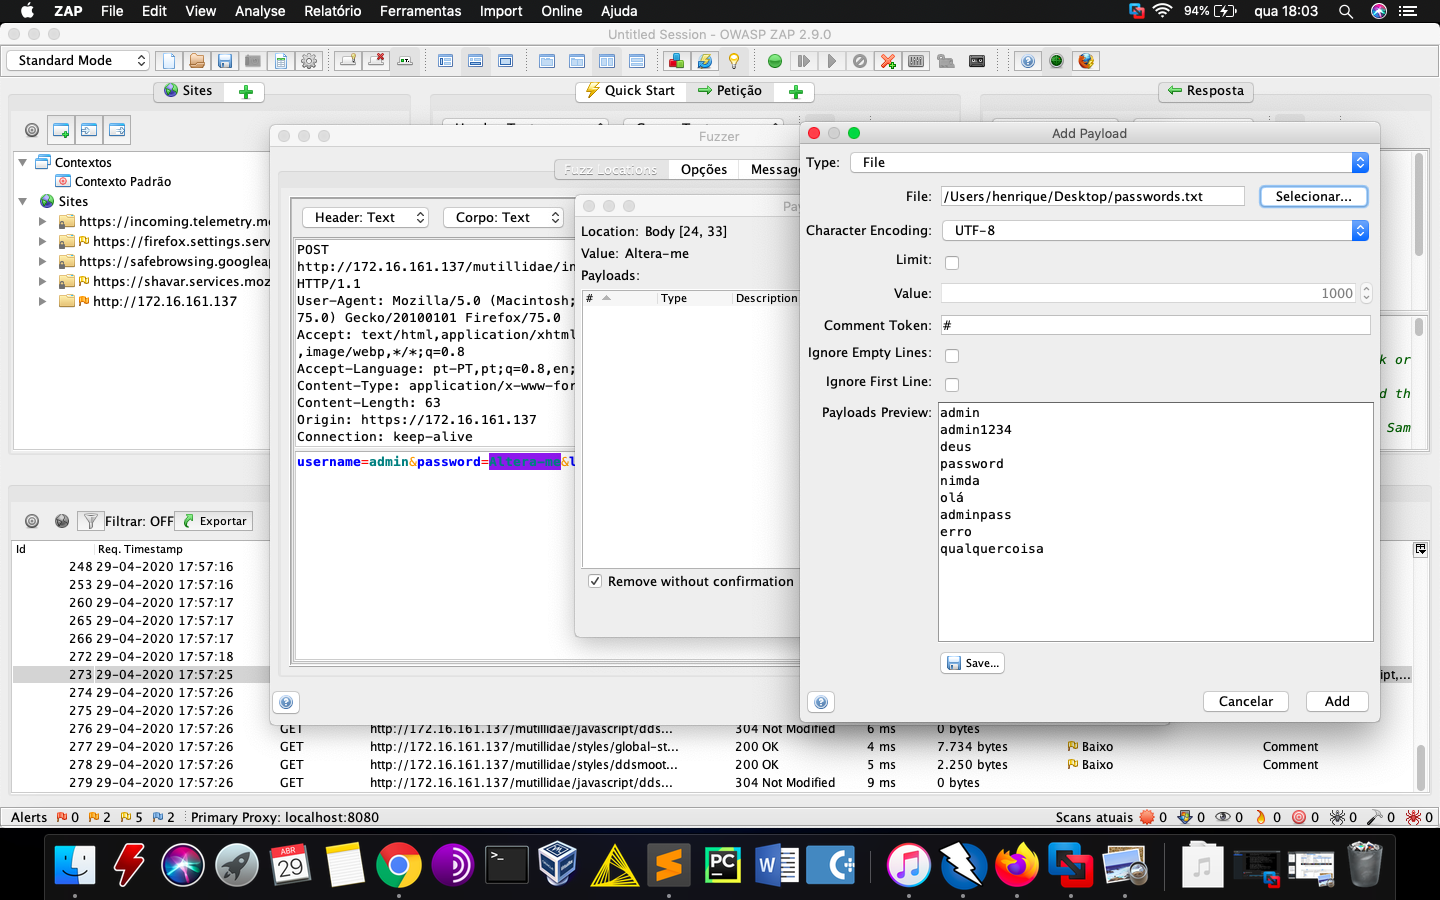
\includegraphics[scale = 0.31]{fig30.png}

  \caption{Configuração do Fuzzer para usar ficheiro pré-gerado de possíveis passwords}

\end{figure}

Para termos uma forma de validação mais simples, caso a password esteja correta, podemos na tab opções escolher "Follow Redirect" para que mal haja uma mudança de página, ou seja, a password inserida foi a correta ou despoletou uma ação que nos levou a uma página diferente, o ZAP pare o scan e possamos observar como o último pacote enviado foi preenchido. Assim podemos tentar substituir a password no site e verificar se é a password correta ou não.

\begin{figure}[H]

  \centering

  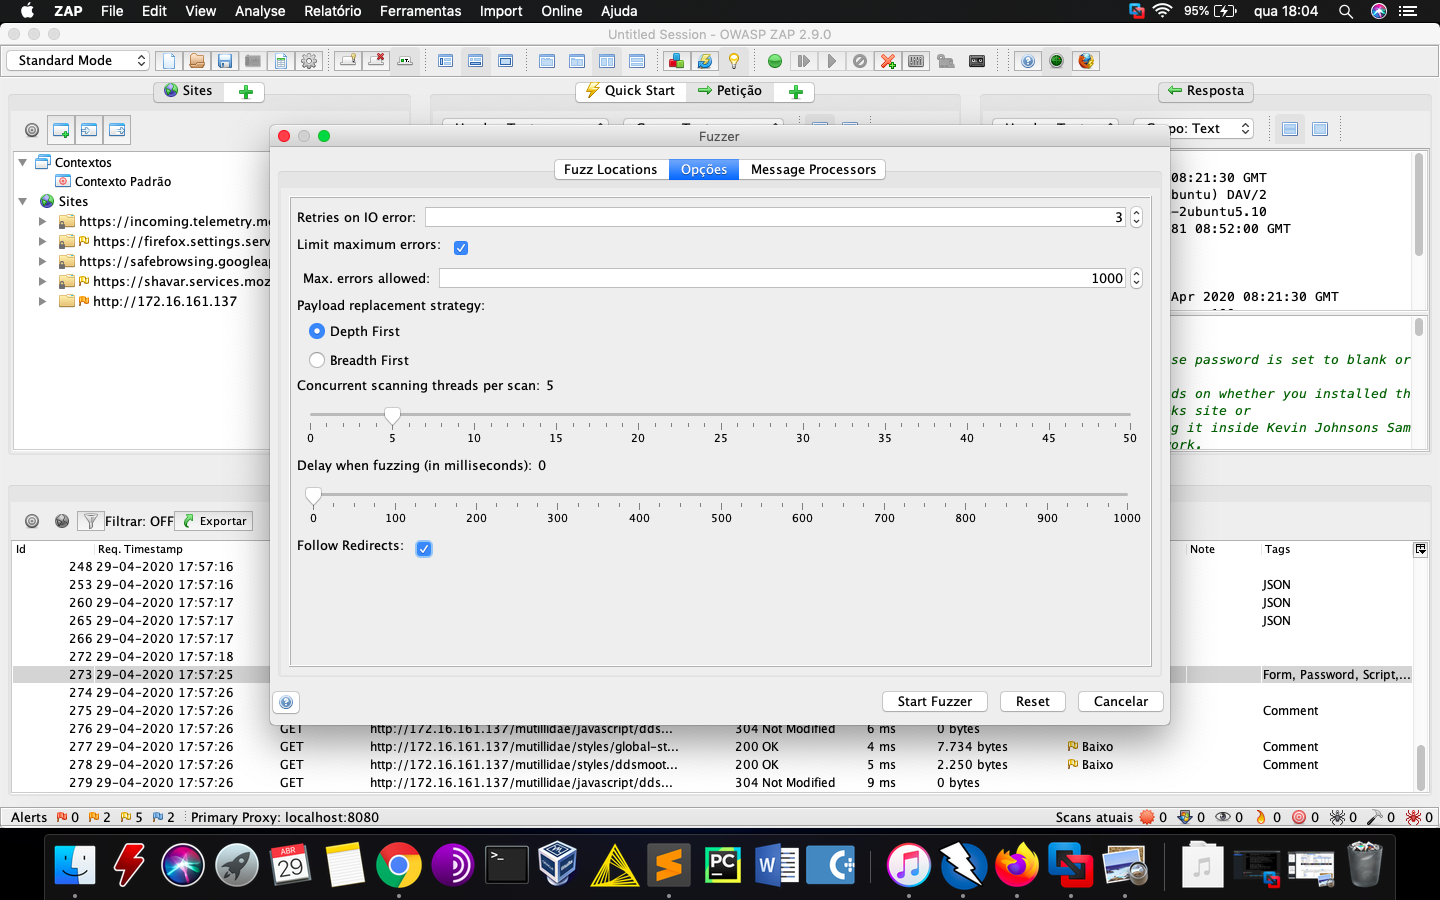
\includegraphics[scale = 0.31]{fig31.png}

  \caption{Configuração para parar no primeiro redirecionamento}

\end{figure}
\begin{figure}[H]

  \centering

  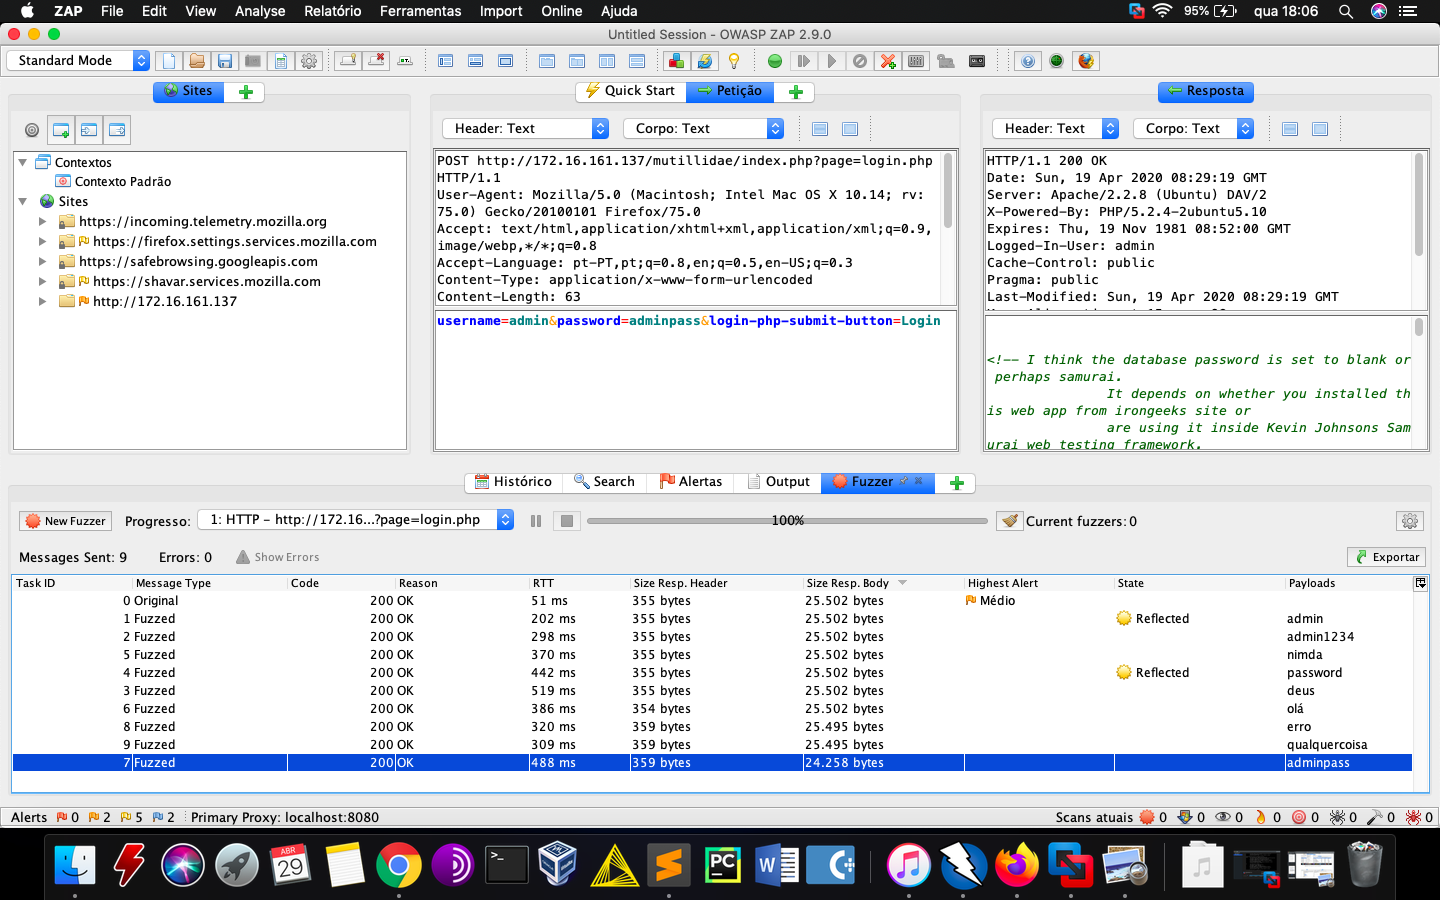
\includegraphics[scale = 0.31]{fig32.png}

  \caption{Resultado em que a página foi redirecionada}

\end{figure}
 Na imagem acima podemos ver que o payload do campo password foi preenchido com a palavra \textit{adminpass}, assim ao testarmos na página confirmamos que de facto esta é a password correta.

\begin{figure}[H]

  \centering

  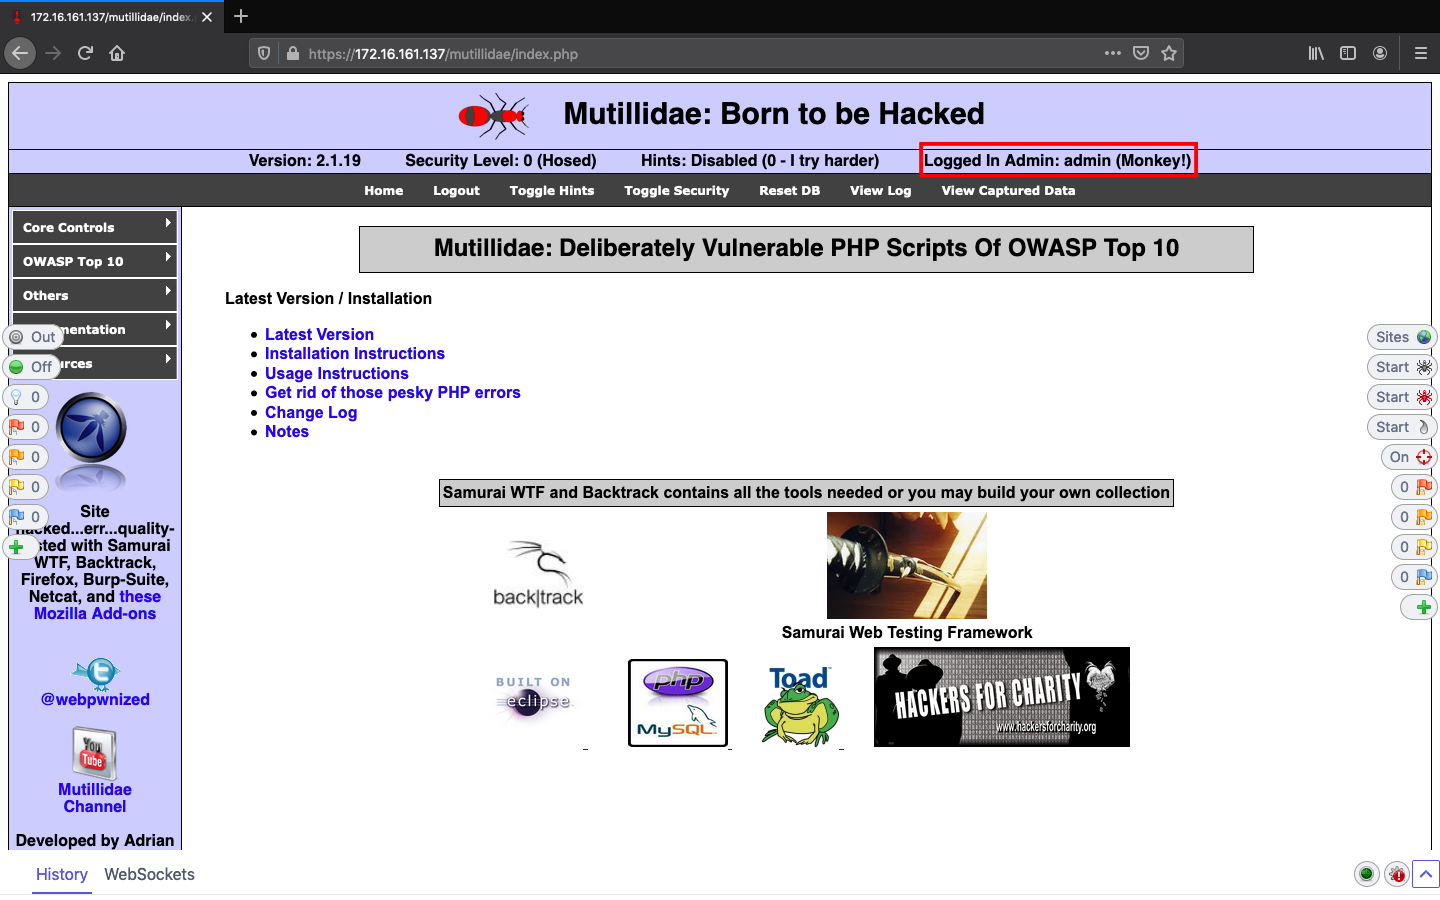
\includegraphics[scale = 0.31]{fig33.png}

  \caption{Resultadod do teste do resultado anterior no site}

\end{figure}


%################################## CROSS SITE SCRIPTING ########################################


\subsubsection{Cross Site Scripting}

Neste teste vamos focar-nos em realizar o ataque quando o utilizador efetua o login.
Fazendo uso do ZAP é possivel efetuar um breakpoint nos pedidos do utilizador e nas respostas recebidas. A imagem seguinte mostra o pedido de autenticação do utilizador.

\begin{figure}[H]

  \centering

  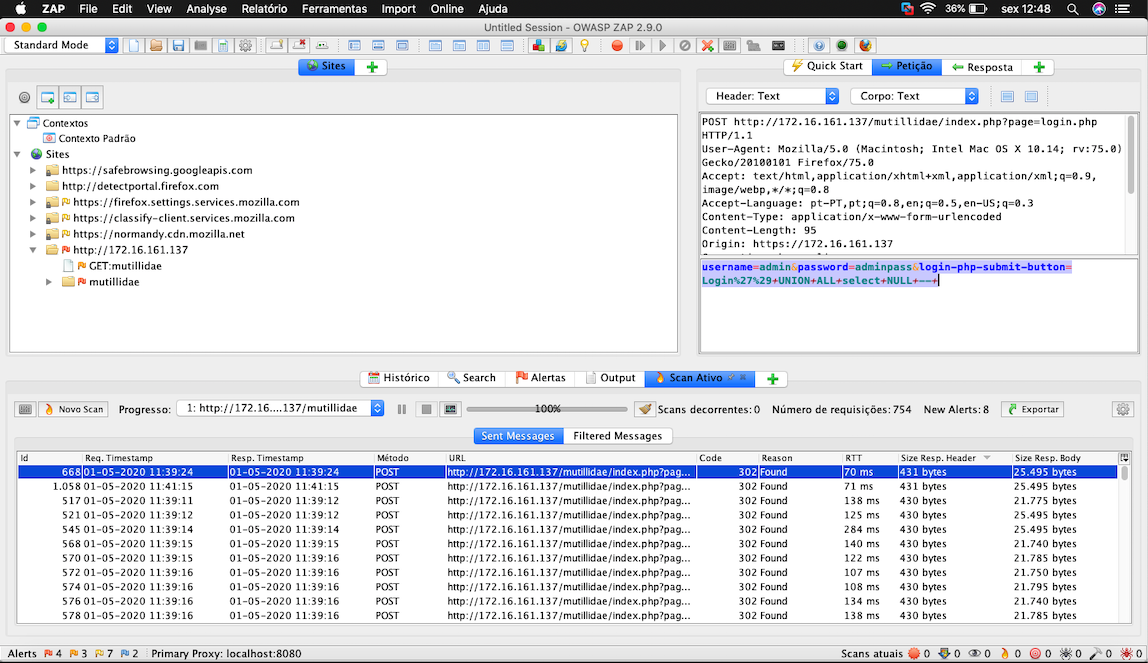
\includegraphics[scale = 0.31]{fig45.png}

  \caption{Pedido de autenticação do utilizador}

\end{figure}



Este ataque consiste portanto, em tentar alterar os campos enviados pelo utilizador para realizar este ataque.\newline
Neste caso, vamos usar o Fuzzer para modificar o campo do username com as opções XSS: URI Cross Site Scripting, XSS Style injection e XSS XML injection\footnote[1]{ Note-se que são apenas algumas opções, todas as opções apresentadas pelo ZAP são válidas.}.
\begin{figure}[H]

  \centering

  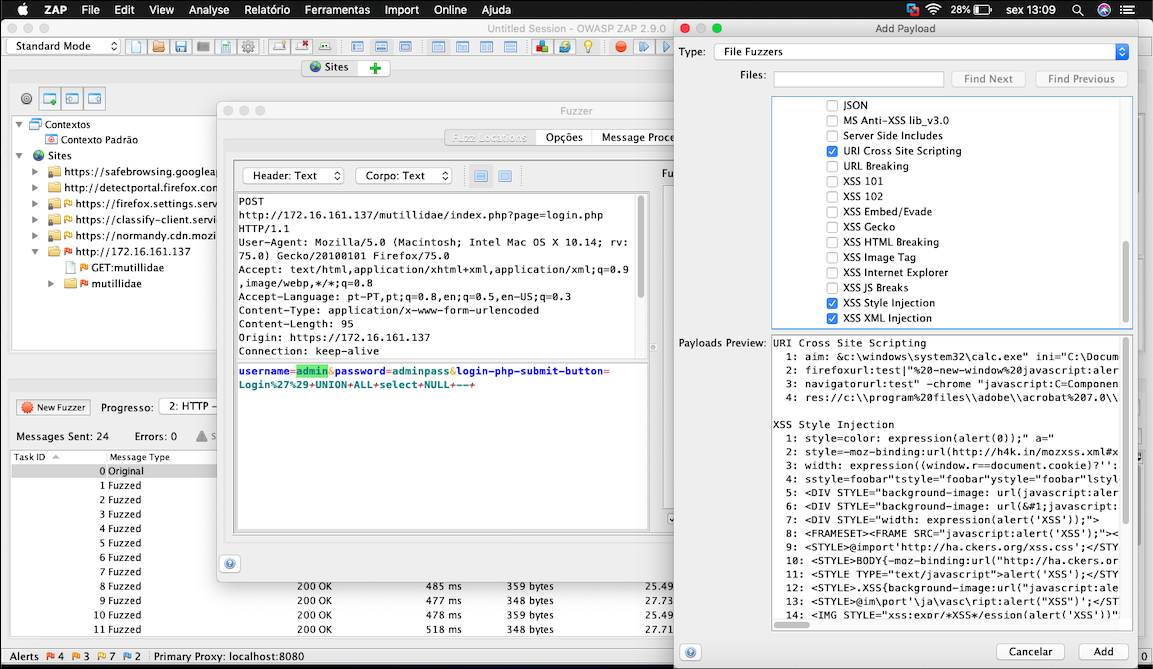
\includegraphics[scale = 0.31]{fig46.png}

  \caption{Opções de configuração do Fuzzer}

\end{figure}


 Se observarmos agora os resultados do ZAP vemos que Aparecem alguns simbolos amarelos como a nota reflected ao lado. Estes são os ataques que foram bem sucedidos na injeção de código malicioso no campo do username.

\begin{figure}[H]

  \centering

  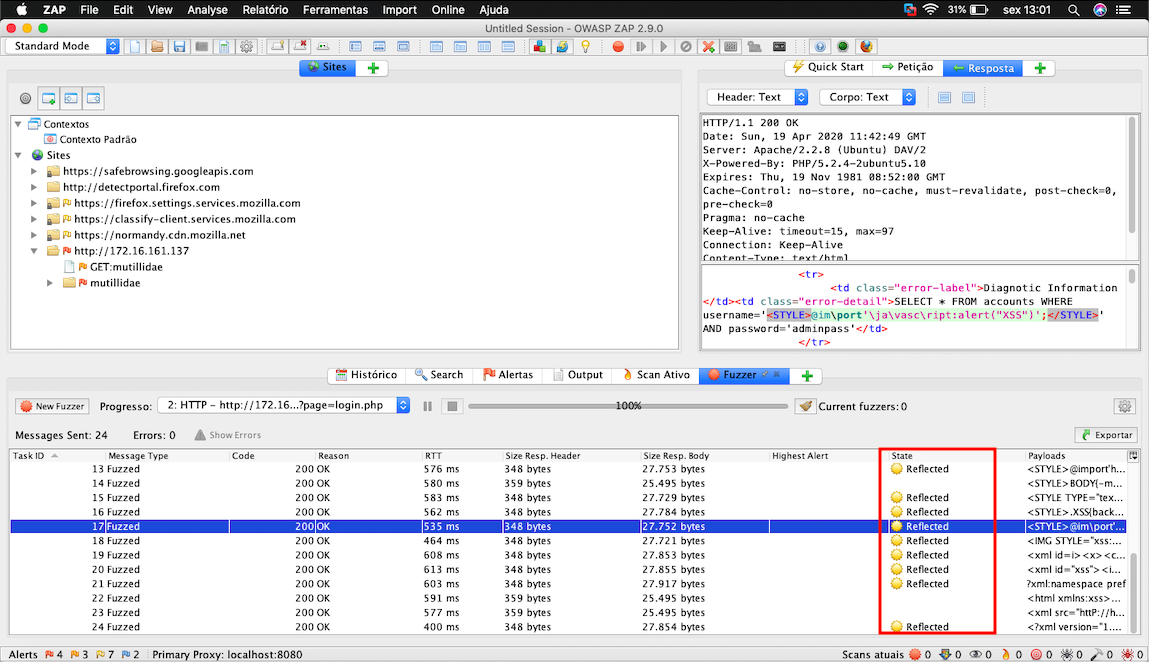
\includegraphics[scale = 0.31]{fig47.png}

  \caption{Resultados de injeção de código no campo username}

\end{figure}

Vamos então verificar o resultado no lado do utilizador caso trocassemos o campo username por um dos payloads possiveis que foram redirecionados. Neste caso para melhor visualização vamos usar o seguinte código: \textit{<script>alert('XSS');</script>}

\begin{figure}[H]

  \centering

  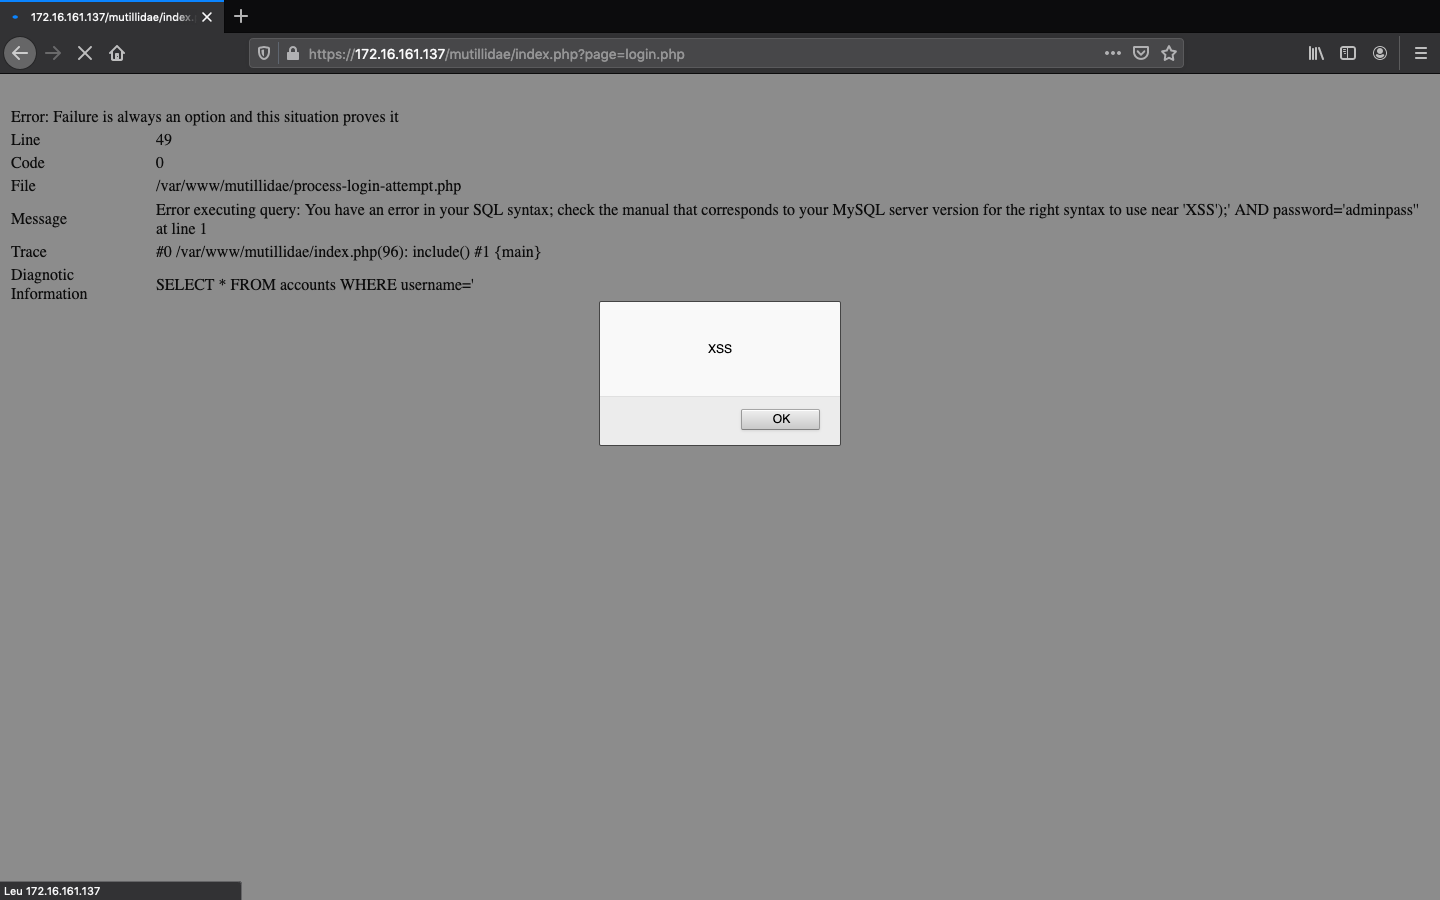
\includegraphics[scale = 0.31]{fig48.png}

  \caption{Teste de utilização de um dos payloads}

\end{figure}

%###################################### HIDDEN FILES ############################################





\subsubsection{Obter ficheiros escondidos no Servidor}

Neste ataque nós pretendemos descobrir ficheiros escondidos no servidor do site. Para isso podemos utilizar a opção "force browse directory (and children)". Nós utilizamos esta opção uma vez que a opção "force browse directory" não mostra tudo o que encontra.
\begin{figure}[H]

  \centering

  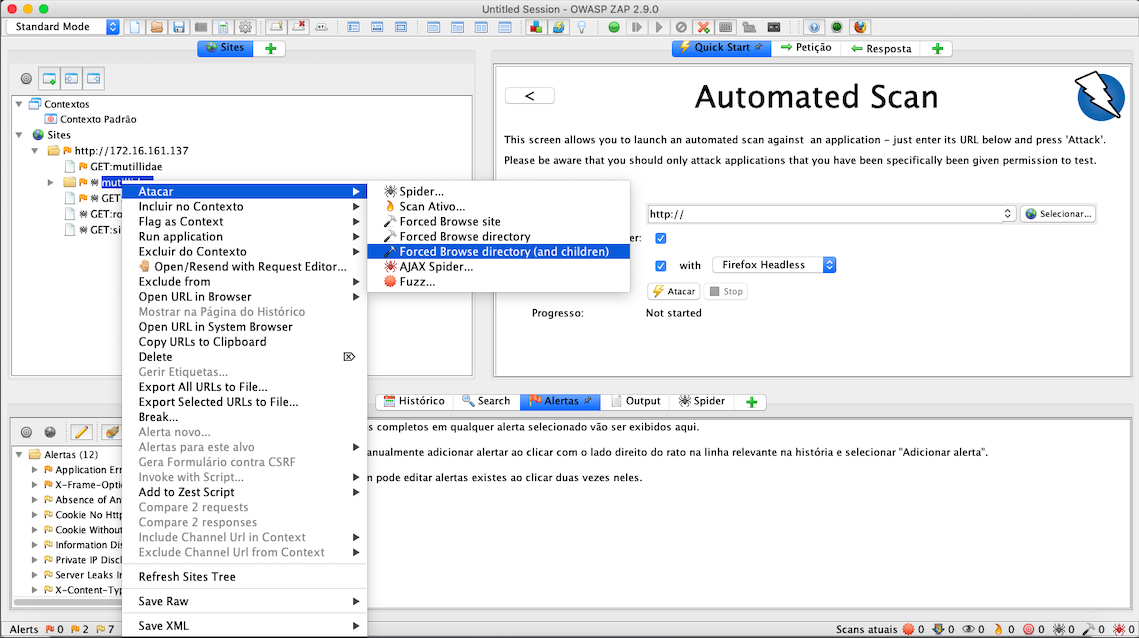
\includegraphics[scale = 0.31]{fig13.png}

  \caption{Procedimento de escolha de browse directory}

\end{figure}

É então aberta uma janela como se vê na figura seguinte. Onde selecionamos a lista que vem por defeito com o ZAP que este usará como base para uma estratégia "brute force" onde tentará encontrar os ficheros escondidos listando-os. Em baixo podemos ver o resultado da procura.
\begin{figure}[H]

  \centering

  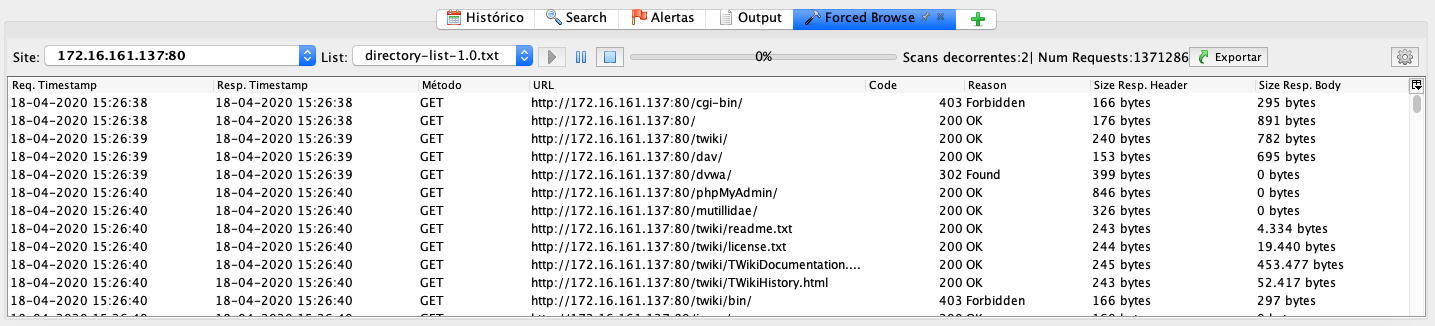
\includegraphics[scale = 0.31]{fig14.png}

  \caption{Resultados da procura}

\end{figure}

Os resultados encontrados são listados como se pode ver na figura assim com vários código associados:

-200  Ok
-403  Forbiden
-302  Found/Moved
-400  Bad Request
-500  Internal Server Error


É no entanto mais facil procurar na janela associada aos pedidos "Get" por palavras chave tais como password ou node como se pode verificar na seguinte figura e posteriormente inspecionar o conteúdo encontrado abrindo uma janela no firefox através do ZAP ou lendo o endereço do pedido get feito e inserindo o url diretamente no firefox obtendo, neste caso, uma lista de usernames e as respetivas passwords.

\begin{figure}[H]

  \centering

  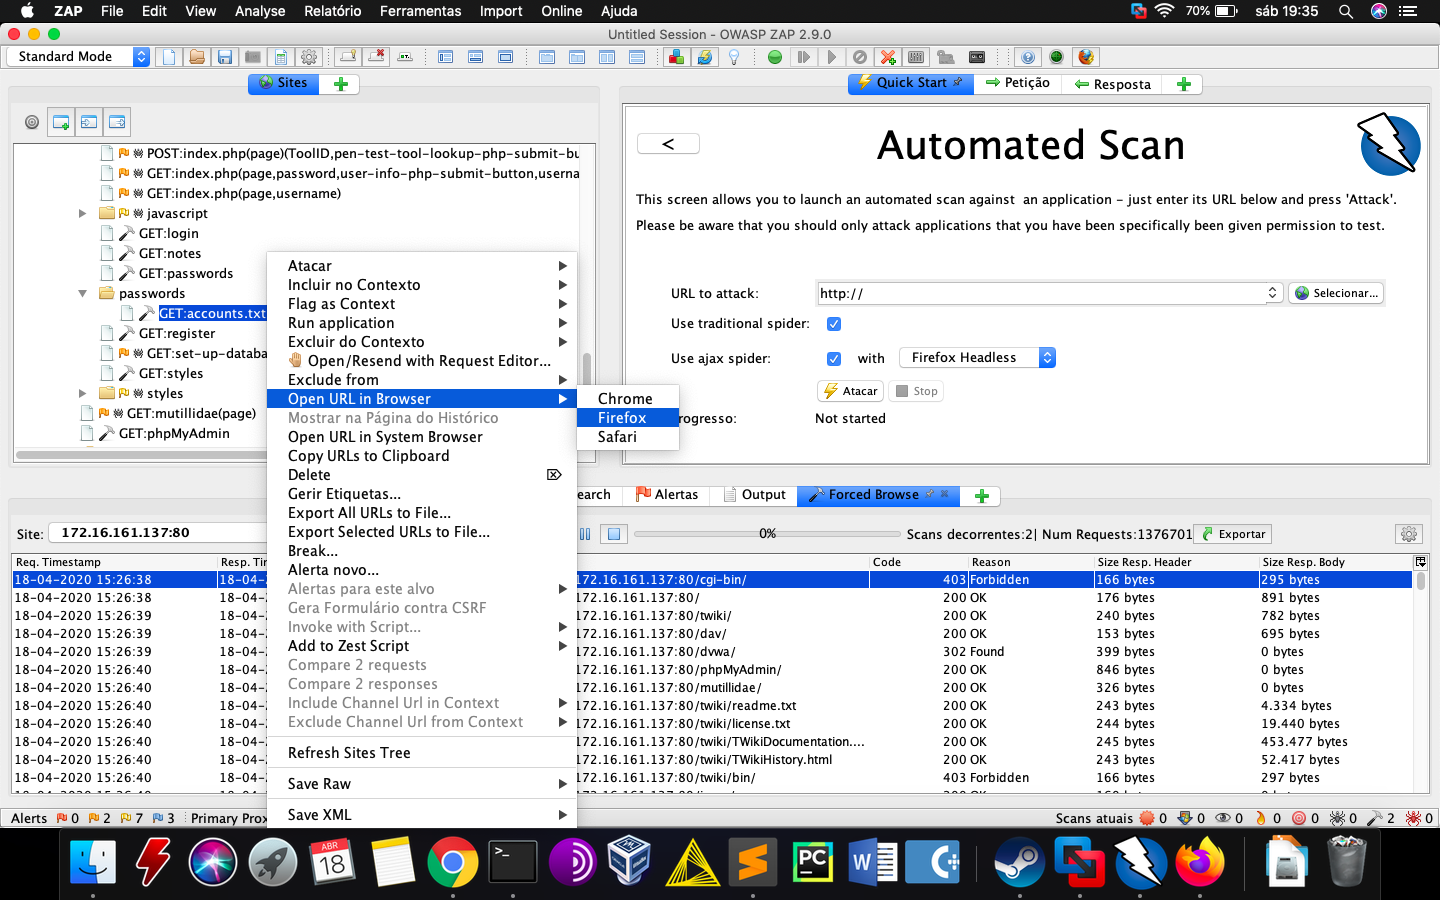
\includegraphics[scale = 0.31]{fig15_1.png}

  \caption{Abertura do URL proibido através do ZAP}

\end{figure}
\begin{figure}[H]

  \centering

  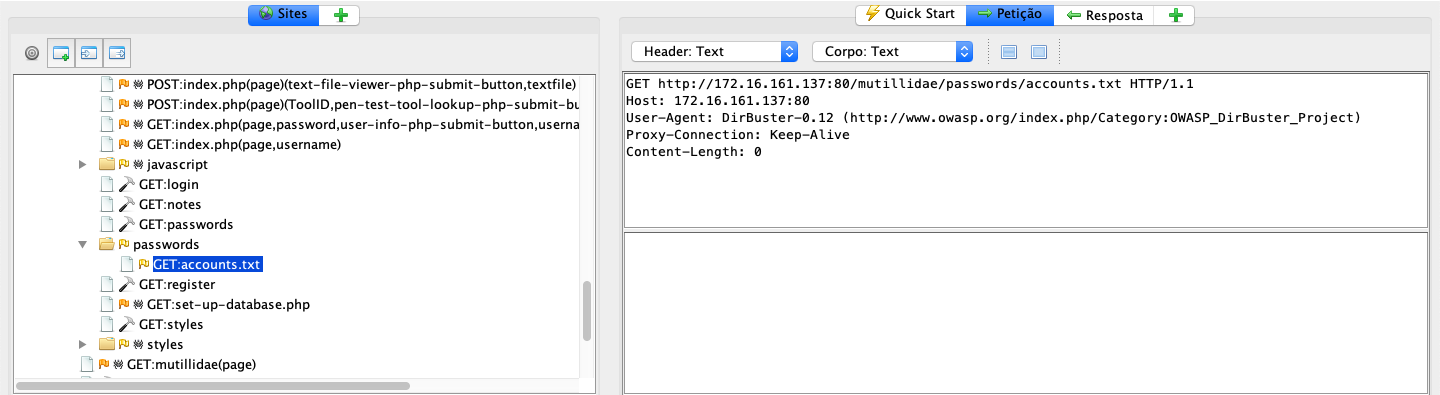
\includegraphics[scale = 0.31]{fig15_2.png}

  \caption{Pedido com o URL proibido}

\end{figure}
\begin{figure}[H]

  \centering

  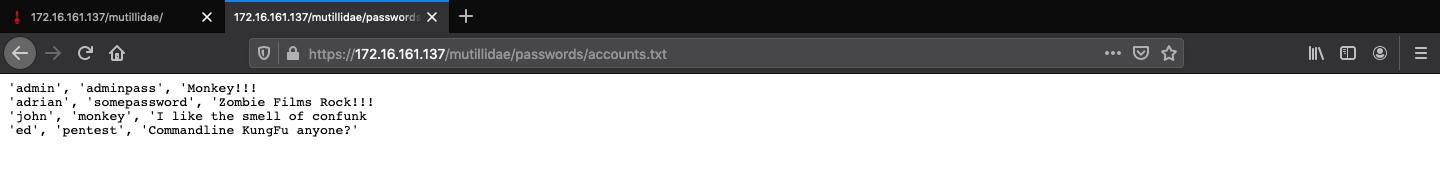
\includegraphics[scale = 0.31]{fig16.png}

  \caption{Resultado da abertura do URL desprotegido}

\end{figure}

